{\color{gray}\hrule}
\begin{center}
\section{Methodology}
\textbf{Systematic Procedure for Paper Selection}
\bigskip
\end{center}
{\color{gray}\hrule}
\begin{multicols}{2}
The research process began by defining our scope together with our supervisor, Professor Jean-Marc Pierson. We focused on creating a state-of-the-art review addressing energy consumption optimization within Container and Cloud Computing.

Initially, we defined a structured "Search Pipeline" illustrated in Figure~\ref{fig:search_pipeline}, ensuring systematic identification and evaluation of relevant papers.

\begin{figure}[H]
    \centering
    \includegraphics[width=0.7\columnwidth]{flowchartTIR.png}
    \caption{Search Pipeline Flowchart}
    \label{fig:search_pipeline}
\end{figure}

We developed an initial search query: \textit{((energy OR resource) AND container)}, including "resource" to account for better resource utilization directly influencing energy efficiency.

Clear exclusion criteria were established beforehand (Table~\ref{tab:Exclusion Rules}), filtering out irrelevant work and focusing exclusively on impactful research.

\begin{table}[H]
\centering
\begin{tabular}{c}
\hline
Direct Exclusion of Paper If \\ \hline
Work is not in English \\ 
Work is not a scientific paper \\ 
Work has fewer than 10 citations \\ 
Work is not related to containers/cloud \\ \hline
\end{tabular}
    \caption{Exclusion Criteria}
    \label{tab:Exclusion Rules}
\end{table}

This approach yielded 34 relevant papers, sourced across various publishers, as depicted in Figure~\ref{fig:exported_papers}.

\begin{figure}[H]
    \centering
    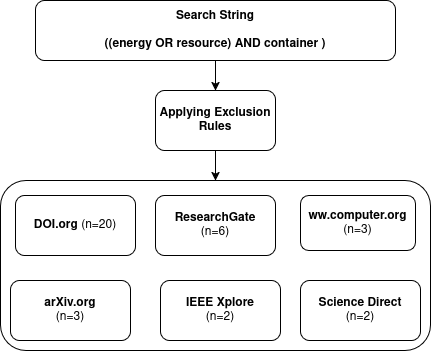
\includegraphics[width=\columnwidth]{sections/exportedPapers.png}
    \caption{Distribution of Exported Papers by Publisher}
    \label{fig:exported_papers}
\end{figure}

The majority of selected studies were published between 2017 and 2019 (Figure~\ref{fig:papers_per_year}), reflecting a peak period of research interest.

\begin{figure}[H]
    \centering
    \includegraphics[width=0.8\columnwidth]{papers_per_year.png}
    \caption{Papers per Year}
    \label{fig:papers_per_year}
\end{figure}

After paper selection, we defined specific classification metrics (Table~\ref{tab:Paper Classification}) to analyze the technical dimensions of energy-aware scheduling approaches.

\begin{table}[H]
\centering
\begin{tabular}{c}
\hline
Classification Categories\\ \hline
Optimization Technique \\ 
Target Level  \\ 
Scheduling Scope \\ 
Energy Strategy \\
Docker Awareness \\
\hline
\end{tabular}
    \caption{Paper Classification Metrics}
    \label{tab:Paper Classification}
\end{table}

The classification categories are defined as follows:

\begin{itemize}
  \small
  \item \textbf{Scheduling Scope}
    \begin{itemize}
      \item \textbf{Online}: Decisions at runtime.
      \item \textbf{Offline}: Known workload beforehand.
      \item \textbf{Predictive}: Forecast-based decisions.
      \item \textbf{Reactive}: Triggered by SLA violations or thresholds.
      \item \textbf{Concurrent}: Simultaneous multiple-task scheduling.
    \end{itemize}

  \item \textbf{Optimization Technique}
    \begin{itemize}
      \item \textbf{Greedy}: Stepwise local decisions.
      \item \textbf{Model-Based}: Predictive analytical models.
      \item \textbf{PSO}: Bio-inspired global optimization.
      \item \textbf{Evolutionary}: Genetic/evolution-based methods.
      \item \textbf{Meta-Heuristic}: High-level heuristic strategies.
      \item \textbf{MCMF}: Flow-network optimization.
    \end{itemize}

  \item \textbf{Energy Strategy}
    \begin{itemize}
      \item \textbf{Consolidation}: Migrate to reduce active hosts.
      \item \textbf{Brownout}: Temporarily disable app components.
      \item \textbf{QoS Maintenance}: Energy-saving without SLA violations.
      \item \textbf{Renewable-aware}: Optimize for renewable energy availability.
    \end{itemize}

  \item \textbf{Docker Awareness}
    \begin{itemize}
      \item \textbf{Pre-Docker}: Pre-containerization (VM-only).
      \item \textbf{Early Docker}: Containers used like VMs.
      \item \textbf{Mature Docker}: Container-specific optimizations.
    \end{itemize}
\end{itemize}

We incorporated \textbf{Docker Awareness} to highlight the technological transition from virtual machines to containers, essential for understanding changes in scheduling complexity. \textbf{Energy Awareness} is included to represent approaches' capability to balance energy efficiency with QoS constraints, recognizing the different trade-offs between performance and sustainability.

Finally, Tables~\ref{tab:technical_papers} and \ref{tab:surveys} summarize our classified selection, and Figure~\ref{fig:trend_analysis} visually correlates scheduling approaches with their publication years.

\begin{figure}[H]
    \centering
    \includegraphics[width=1\linewidth]{Trend_Analysis.jpeg}
    \caption{Trend Analysis}
    \label{fig:trend_analysis}
\end{figure}

\end{multicols}

\begin{footnotesize}
\begin{longtable}{|p{3.8cm}|p{2.3cm}|p{1.6cm}|p{2.3cm}|p{2.2cm}|p{2cm}|}
\hline
\textbf{Paper Ref.} & \textbf{Optimization Technique} & \textbf{Target Level} & \textbf{Scheduling Scope} & \textbf{Energy Strategy} & \textbf{Docker Awareness} \\
\hline
\endfirsthead

\hline
\textbf{Paper Ref.} & \textbf{Optimization Technique} & \textbf{Target Level} & \textbf{Scheduling Scope} & \textbf{Energy Strategy} & \textbf{Docker Awareness} \\
\hline
\endhead

Availability-Aware Scheduler\cite{alahmad_availability-aware_2018} (2018) & Greedy & Container, VM & Offline & Availability & Mature Docker\\
\hline
Renewable-Aware Scheduling\cite{kumar_renewable_2019} (2019)& Greedy & Container, VM & Reactive & Consolidation & Mature Docker \\
\hline
Concurrent Container Scheduling\cite{hu_concurrent_2020} (2020)& MCMF & Container & Concurrent & Consolidation & Mature Docker \\
\hline
GP Hyper-Heuristic for Containers\cite{tan_hybrid_2019} (2019)& Evolutionary & Container, VM & Online & Consolidation & Mature Docker \\
\hline
PSO-Based Container Consolidation\cite{shi_energy-aware_2018} (2018)& PSO & Container & Offline & Consolidation & Mature Docker \\
\hline
Energy-Efficient Container Framework\cite{piraghaj_framework_2015} (2015)& Greedy & Container, VM & Reactive & Consolidation & Early Docker \\
\hline
VM Consolidation Strategy\cite{carrega_energy-aware_2017} (2017)& Meta-Heuristic & VM & Online & Consolidation & Mature Docker \\
\hline
Predictive Resource Provisioning\cite{dabbagh_energy-efficient_2015} (2015)& Model-based  & VM & Predictive & Consolidation & Early-Docker \\
\hline
Dynamic VM Reallocation\cite{beloglazov_energy_2010} (2010) & Greedy & VM & Online & Consolidation & Pre-Docker \\
\hline
Autonomic Container Management\cite{barna_delivering_2017} (2017) & Model-based & Container, VM & Predictive & QoS & Mature Docker \\
\hline
Brownout-Based Scheduling\cite{xu_energy_2016} (2016)& Greedy & Application Layer & Reactive & Brownout & Mature Docker \\
\hline
GPR + Convex VM Planning\cite{bui_energy_2017} (2017) & Model-Based & VM, PM & Predictive & Consolidation & Mature Docker \\
\hline
SLA-Aware Consolidation\cite{li_sla-aware_2018} (2018) & Model-Based & VM, PM & Predictive & Consolidation & Mature Docker \\
\hline
\caption{Classification of Technical Papers on Energy-Aware Scheduling}
\label{tab:technical_papers}
\end{longtable}
\end{footnotesize}

\begin{table}[H]
\centering
\footnotesize
\begin{tabular}{|p{5.5cm}|p{3.5cm}|p{4cm}|}
\hline
\textbf{Paper Ref.} & \textbf{Type} & \textbf{Scope / Focus} \\
\hline
Survey on Energy-Aware Scheduling\cite{hameed_survey_2016}  & Survey & Overview of VM and container-level techniques \\
\hline
Global Energy Estimates\cite{masanet_2020} & Analysis & Environmental impact of data centers \\
\hline
Cloud Impact on Energy\cite{hintemann_2022} & Report & Energy use in European data centers \\
\hline
IEA Report on Data Centers\cite{IEADataCentres} & Report & Global energy trends in ICT and data centers \\
\hline
EU Data Center Energy Trends\cite{avgerinou_trends_2017} & Analysis & EU-level trends in ICT energy consumption \\
\hline
\end{tabular}
\caption{Survey and Analysis Papers}
\label{tab:surveys}
\end{table}







